% !TeX document-id = {d42653b9-9ea4-48c2-860b-3d6e6e9d8ab0}
% !TeX TXS-program:compile = txs:///pdflatex/[--shell-escape]
\documentclass[12pt]{article} % For LaTeX2e
%\usepackage{neurips_2021}
\usepackage[colorlinks, citecolor={blue}]{hyperref}
\usepackage{url}
\usepackage{amsfonts,amscd,amssymb}
\usepackage{amsthm,amsmath,natbib}
\usepackage{mathtools}
\DeclarePairedDelimiter{\ceil}{\lceil}{\rceil}
\usepackage{algorithm2e}
\usepackage{bm}
\usepackage{bbm} %bb font numbers
\usepackage[table]{xcolor}
\usepackage{verbatim}
\usepackage{graphicx}
\usepackage{setspace}
\usepackage{natbib}
\usepackage[margin=1in]{geometry}
\usepackage{enumitem}
%\usepackage[nolists]{endfloat}
\usepackage{listings}
\usepackage[textsize=tiny]{todonotes}
\usepackage{tikz}
\usetikzlibrary{shapes.misc}
\usepackage{etoolbox}
\usepackage{appendix}
\usepackage[format=plain,
labelfont={it},
textfont=it]{caption}
\usepackage{subcaption}
\usepackage{wrapfig}
\usepackage{xr}
\usepackage{booktabs}
\usepackage{multirow}
\usepackage{authblk}
\usepackage{mathbbol}
\usepackage{braket}



\usetikzlibrary{matrix}
\usetikzlibrary{backgrounds}
\usetikzlibrary{calc}
\usetikzlibrary{arrows,shapes}
\usetikzlibrary{decorations}
\usetikzlibrary{decorations.pathmorphing}
\usetikzlibrary{fit}
\usetikzlibrary{decorations.pathreplacing}

\newtoggle{quickdraw}
\toggletrue{quickdraw} % Uncomment this to render more quickly (non-random)


\definecolor{lightgrey}{rgb}{0.9,0.9,0.9}
\definecolor{darkgreen}{rgb}{0,0.3,0}
%\definecolor{darkred}{rgb}{0.3,0,0}

\definecolorset{rgb}{}{}{darkred,0.8,0,0;darkgreen,0,0.5,0;darkblue,0,0,0.5}

%\doublespacing

\SetKwComment{Comment}{/* }{ */}
%\RestyleAlgo{ruled}

\newtheorem{thm}{Theorem}
\newtheorem{lemma}{Lemma}
\newtheorem{prop}{Proposition}
\newtheorem{cor}{Corollary}
\newtheorem{remark}{Remark}
\newtheorem{example}{Example}
\newtheorem{mydef}{Definition}
\newtheorem*{assumption}{Assumption}
\newtheorem{clm}{Claim}

\newcommand{\argmax}{\operatornamewithlimits{arg\,max}}
\newcommand{\argmin}{\operatornamewithlimits{arg\,min}}
\newcommand*{\fplus}{\genfrac{}{}{0pt}{}{}{+}}
\newcommand*{\fdots}{\genfrac{}{}{0pt}{}{}{\cdots}}
\newcommand{\mb}{\mathbf}
\newcommand{\mc}{\mathcal}
\newcommand{\dx}{\mbox{d}}

\renewcommand{\vec}[1]{\mathbf{#1}}
\newcommand{\numTaxa}{N}
\newcommand{\numTraits}{D}
\newcommand{\numDatasets}{M}
%\newcommand{\numLatent}{D}
\newcommand{\taxonIndex}{i}
\newcommand{\traitIndex}{j}
\newcommand{\traitData}{\vec{Y}}
\newcommand{\traitDatum}{y}
\newcommand{\datasetIndex}{m}
\newcommand{\exemplar}{\text{e}}

\newcommand{\sequences}{\vec{S}}
\newcommand{\latentData}{\vec{X}}
\newcommand{\latentdata}{\vec{x}}
\newcommand{\latentDatum}{x}
\newcommand{\phylogeneticParameters}{\boldsymbol{\phi}}
\newcommand{\phylogeny}{{\cal G}}
\newcommand{\tree}{\phylogeny}
%\newcommand{\otherParameters}{\boldsymbol{\
\newcommand{\transpose}{^{t}}

\newcommand{\distanceMatrix}{\mathbf{Y}}
\newcommand{\distance}{y}
\newcommand{\summant}{r}



\newcommand{\cdensity}[2]{\ensuremath{p(#1 \,|\,#2)}}
\newcommand{\density}[1]{\ensuremath{p(#1 )}}

\newcommand{\treeNode}{\nu}

\newcommand{\traitVariance}{\mathbf{\Sigma}}
\newcommand{\nodeIndex}{c}

%\newcommand{\parent}[1]{\mbox{\tiny pa}(#1)}
\newcommand{\parentBig}[1]{\mbox{pa}(#1)}

\newcommand{\sibling}[1]{\mbox{\tiny sib}(#1)}
\newcommand{\siblingBig}[1]{\mbox{sib}(#1)}

\newcommand{\rootMean}{\boldsymbol{\mu}_0}
\newcommand{\rootVarianceScalar}{\tau_0}
\newcommand{\unsequencedVarianceScalar}{\tau_{\exemplar}}
\newcommand{\treeVariance}{\vec{V}_{\tree}}
\newcommand{\hatTreeVariance}{\hat{\vec{V}}_{\tree}}
\newcommand{\mdsSD}{\sigma}
\newcommand{\mdsVariance}{\mdsSD^2}
\newcommand{\residual}{\hat{\traitDatum}}
\newcommand{\modelDistance}{\delta}
\newcommand{\cdf}{\phi}
\newcommand{\normalCDF}[1]{\Phi \left( #1 \right)}

\newcommand{\order}[1]{{\cal O}\hspace{-0.2em}\left( #1 \right)}

\newcommand{\rootNode}{\nu^{\datasetIndex}_{2 \numTaxa_{\datasetIndex} -1 }}
\newcommand{\pathLength}[1]{d(F, #1 )}
\newcommand{\pathLengthNew}[2]{
d_{F}
(
{#1}, {#2}
)
}
\newcommand{\J}{\vec{J}}
\newcommand{\pprime}{^{\prime}}
\newcommand{\otherIndex}{i \pprime}
\def\kronecker{\raisebox{1pt}{\ensuremath{\:\otimes\:}}}

\definecolor{trevorblue}{rgb}{0.330, 0.484, 0.828}
\definecolor{trevoryellow}{rgb}{0.829, 0.680, 0.306}

%%%
%% LaTeX source to reference manuscript changes in revision letters
%%
%% In the manuscript file:
%% 1. Include this file 
%%      %%
%% LaTeX source to reference manuscript changes in revision letters
%%
%% In the manuscript file:
%% 1. Include this file 
%%      %%
%% LaTeX source to reference manuscript changes in revision letters
%%
%% In the manuscript file:
%% 1. Include this file 
%%      \input{make-edits}
%% 2. Define manuscript modifications as
%%      \myedit{UniqueLabel}{Text to appear in manuscript and revision letter}
%%
%% In the revision letter file:
%% 1. Include the automatically updated modifications file
%%      \input{jobname.xtr}
%% 2. Include modified text with
%%      \myeditUniqueLabel
%%
%% Marc A. Suchard
%% 24-Jul-2006
%%

\newwrite\XTR
\AtBeginDocument{\immediate\openout\XTR\jobname.xtr}
\AtEndDocument{\immediate\closeout\XTR}

\newcommand{\myedit}[2]{ % first options is a label, second options is the text
\parbox{0em}{
\shipout\box1{
  \def\mynamea{myedit#1}
  \def\mynameb{\csname \mynamea\endcsname}
\write\XTR{
      \string\newcommand
{\csname myedit#1\endcsname}
}
\write\XTR{
         {``\expandafter\string#2''
         (pg.\string~\thepage)}
}
%\write\XTR{
%    (pg.\string~\thepage)
%}
}
%\hspace*{-1in}
}
%
%\def\thistext{\noexpand#2}
%  \immediate\write\XTR{
%   %     \begin{verbatim}
%        \thistext
%   %     \end{verbatim}
%  }
%\endgroup
%}
%\shipout\vbox{0}
%        \label{\expand\mylabel}
%        \thepage
%  \mylabel
%  \hspace*{-0em}
%  {\bf#2}
#2
}

\newcommand{\myeditblank}[2]{ % first options is a label, second options is the text
\parbox{1em}{
\shipout\box1{
  \def\mynamea{myedit#1}
  \def\mynameb{\csname \mynamea\endcsname}
\write\XTR{
      \string\newcommand
{\csname myedit#1\endcsname}
}
\write\XTR{
         {\expandafter\string#2
         (pg.\string~\thepage)}
}
%\write\XTR{
%    (pg.\string~\thepage)
%}
}
%\hspace*{-1in}
}
%
%\def\thistext{\noexpand#2}
%  \immediate\write\XTR{
%   %     \begin{verbatim}
%        \thistext
%   %     \end{verbatim}
%  }
%\endgroup
%}
%\shipout\vbox{0}
%        \label{\expand\mylabel}
%        \thepage
%  \mylabel
%  \hspace*{-1em}
%  {\bf#2}
}



%\newlength{\strikewidth}
%\newlength{\strikelength}
%\setlength{\strikewidth}{1pt}

%\newcommand{\remove}[1]{
%    \settowidth{\strikelength}{#1}
%    #1\hspace{-\strikelength}
%    \rule[0.5ex]{\strikelength}{\strikewidth}
%}

%\usepackage{ulem}
%\newcommand{\remove}[1]{\sout{#1}}
\newcommand{\remove}[1]{\hspace*{-1em}}

\newcommand{\add}[1]{
%        {\bf #1}
#1%\hspace*{0em}
}


%% 2. Define manuscript modifications as
%%      \myedit{UniqueLabel}{Text to appear in manuscript and revision letter}
%%
%% In the revision letter file:
%% 1. Include the automatically updated modifications file
%%      \input{jobname.xtr}
%% 2. Include modified text with
%%      \myeditUniqueLabel
%%
%% Marc A. Suchard
%% 24-Jul-2006
%%

\newwrite\XTR
\AtBeginDocument{\immediate\openout\XTR\jobname.xtr}
\AtEndDocument{\immediate\closeout\XTR}

\newcommand{\myedit}[2]{ % first options is a label, second options is the text
\parbox{0em}{
\shipout\box1{
  \def\mynamea{myedit#1}
  \def\mynameb{\csname \mynamea\endcsname}
\write\XTR{
      \string\newcommand
{\csname myedit#1\endcsname}
}
\write\XTR{
         {``\expandafter\string#2''
         (pg.\string~\thepage)}
}
%\write\XTR{
%    (pg.\string~\thepage)
%}
}
%\hspace*{-1in}
}
%
%\def\thistext{\noexpand#2}
%  \immediate\write\XTR{
%   %     \begin{verbatim}
%        \thistext
%   %     \end{verbatim}
%  }
%\endgroup
%}
%\shipout\vbox{0}
%        \label{\expand\mylabel}
%        \thepage
%  \mylabel
%  \hspace*{-0em}
%  {\bf#2}
#2
}

\newcommand{\myeditblank}[2]{ % first options is a label, second options is the text
\parbox{1em}{
\shipout\box1{
  \def\mynamea{myedit#1}
  \def\mynameb{\csname \mynamea\endcsname}
\write\XTR{
      \string\newcommand
{\csname myedit#1\endcsname}
}
\write\XTR{
         {\expandafter\string#2
         (pg.\string~\thepage)}
}
%\write\XTR{
%    (pg.\string~\thepage)
%}
}
%\hspace*{-1in}
}
%
%\def\thistext{\noexpand#2}
%  \immediate\write\XTR{
%   %     \begin{verbatim}
%        \thistext
%   %     \end{verbatim}
%  }
%\endgroup
%}
%\shipout\vbox{0}
%        \label{\expand\mylabel}
%        \thepage
%  \mylabel
%  \hspace*{-1em}
%  {\bf#2}
}



%\newlength{\strikewidth}
%\newlength{\strikelength}
%\setlength{\strikewidth}{1pt}

%\newcommand{\remove}[1]{
%    \settowidth{\strikelength}{#1}
%    #1\hspace{-\strikelength}
%    \rule[0.5ex]{\strikelength}{\strikewidth}
%}

%\usepackage{ulem}
%\newcommand{\remove}[1]{\sout{#1}}
\newcommand{\remove}[1]{\hspace*{-1em}}

\newcommand{\add}[1]{
%        {\bf #1}
#1%\hspace*{0em}
}


%% 2. Define manuscript modifications as
%%      \myedit{UniqueLabel}{Text to appear in manuscript and revision letter}
%%
%% In the revision letter file:
%% 1. Include the automatically updated modifications file
%%      \input{jobname.xtr}
%% 2. Include modified text with
%%      \myeditUniqueLabel
%%
%% Marc A. Suchard
%% 24-Jul-2006
%%

\newwrite\XTR
\AtBeginDocument{\immediate\openout\XTR\jobname.xtr}
\AtEndDocument{\immediate\closeout\XTR}

\newcommand{\myedit}[2]{ % first options is a label, second options is the text
\parbox{0em}{
\shipout\box1{
  \def\mynamea{myedit#1}
  \def\mynameb{\csname \mynamea\endcsname}
\write\XTR{
      \string\newcommand
{\csname myedit#1\endcsname}
}
\write\XTR{
         {``\expandafter\string#2''
         (pg.\string~\thepage)}
}
%\write\XTR{
%    (pg.\string~\thepage)
%}
}
%\hspace*{-1in}
}
%
%\def\thistext{\noexpand#2}
%  \immediate\write\XTR{
%   %     \begin{verbatim}
%        \thistext
%   %     \end{verbatim}
%  }
%\endgroup
%}
%\shipout\vbox{0}
%        \label{\expand\mylabel}
%        \thepage
%  \mylabel
%  \hspace*{-0em}
%  {\bf#2}
#2
}

\newcommand{\myeditblank}[2]{ % first options is a label, second options is the text
\parbox{1em}{
\shipout\box1{
  \def\mynamea{myedit#1}
  \def\mynameb{\csname \mynamea\endcsname}
\write\XTR{
      \string\newcommand
{\csname myedit#1\endcsname}
}
\write\XTR{
         {\expandafter\string#2
         (pg.\string~\thepage)}
}
%\write\XTR{
%    (pg.\string~\thepage)
%}
}
%\hspace*{-1in}
}
%
%\def\thistext{\noexpand#2}
%  \immediate\write\XTR{
%   %     \begin{verbatim}
%        \thistext
%   %     \end{verbatim}
%  }
%\endgroup
%}
%\shipout\vbox{0}
%        \label{\expand\mylabel}
%        \thepage
%  \mylabel
%  \hspace*{-1em}
%  {\bf#2}
}



%\newlength{\strikewidth}
%\newlength{\strikelength}
%\setlength{\strikewidth}{1pt}

%\newcommand{\remove}[1]{
%    \settowidth{\strikelength}{#1}
%    #1\hspace{-\strikelength}
%    \rule[0.5ex]{\strikelength}{\strikewidth}
%}

%\usepackage{ulem}
%\newcommand{\remove}[1]{\sout{#1}}
\newcommand{\remove}[1]{\hspace*{-1em}}

\newcommand{\add}[1]{
%        {\bf #1}
#1%\hspace*{0em}
}


%\makeatletter
%\def\title@font{\Huge}
%\let\ltx@maketitle\@maketitle
%\def\@maketitle{\bgroup%
%	\let\ltx@title\@title%
%	\def\@title{\resizebox{\textwidth}{!}{%
%			\mbox{\title@font\ltx@title}%
%	}}%
%	\ltx@maketitle%
%	\egroup}
%\makeatother


\title{A quantum parallel Markov chain Monte Carlo}
\date{}



\author{Andrew J.~Holbrook}


\affil{UCLA Biostatistics}





\renewcommand\Authands{ and }


\graphicspath{{figures/}}

\begin{document}


\maketitle




\begin{abstract}

We propose a novel quantum computing strategy for \emph{parallel MCMC} algorithms that generate multiple proposals at each step. This strategy makes parallel MCMC amenable to quantum parallelization by using the Gumbel-max trick to turn the generalized accept-reject step into a discrete optimization problem.  This allows us to embed target density evaluations within a well-known extension of Grover's quantum search algorithm.  Letting $P$ denote the number of proposals in a single MCMC iteration, the combined strategy reduces the number of target evaluations required from $\order{P}$ to $\order{P^{1/2}}$.  In the following, we review both the rudiments of quantum computing and the Gumbel-max trick in order to elucidate their combination for as wide a readership as possible. 


\end{abstract}


\section{Introduction}

\newcommand{\ttheta}{\boldsymbol{\theta}}
\newcommand{\dd}{\mbox{d}}
\newcommand{\ppsi}{\boldsymbol{\psi}}
\newcommand{\U}{\mathbf{U}}
\newcommand{\I}{\mathbf{I}}
\renewcommand{\H}{\mathbf{H}}
\newcommand{\A}{\mathbf{A}}
\newcommand{\B}{\mathbf{B}}
\newcommand{\G}{\mathbf{G}}
\newcommand{\ppi}{\boldsymbol{\pi}}
\newcommand{\llambda}{\boldsymbol{\lambda}}

Parallel MCMC techniques use multiple proposals to obtain efficiency gains over MCMC algorithms such as Metropolis-Hastings \citep{metropolis1953equation,hastings1970monte} and its progeny that use only a single proposal.  \citet{neal2003markov} first develops efficient MCMC transitions for inferring the states of hidden Markov models by proposing a `pool' of candidate states and using dynamic programming to select among them. Next, \citet{tjelmeland2004using} considers inference in the general setting and shows how to maintain detailed balance for an arbitrary number $P$ of proposals.  Consider a probability distribution $\pi(\dd\ttheta)$ defined on $\mathbb{R}^D$ that admits a probability density $\pi(\ttheta)$ with respect to the Lebesgue measure, i.e., $\pi(\dd \ttheta)=:\pi(\ttheta)\dd\ttheta$. To generate samples from the target distribution $\pi$, we craft a kernel $P(\ttheta_0,\dd \ttheta)$ that satisfies
\begin{align}\label{eq:fixes}
\pi(A) = \int \pi(\dd \ttheta_0) P(\ttheta_0,A) \, \quad a.s.
\end{align} 
for  $A \subset \mathbb{R}^D$ for which $\pi(A) > 0$.  Letting $\ttheta_0$ denote the current state of the Markov chain, \citet{tjelmeland2004using} proposes sampling from such a kernel $P(\ttheta_0,\cdot)$ by drawing $P$ proposals $\ttheta_1,\dots,\ttheta_P$ from a distribution $Q(\ttheta_0,\dd \ttheta) =: q(\ttheta_0,\ttheta)\dd \ttheta$ and selecting the next Markov chain state from among the current and proposed states with probabilities
\begin{align}\label{eq:probs}
\pi_p = \frac{\pi(\ttheta_p) \prod_{p' \neq p} q(\ttheta_p,\ttheta_{p'})}{\sum_{p''=0}^P \pi(\ttheta_{p''}) \prod_{p' \neq p''} q(\ttheta_{p''},\ttheta_{p'})} \, , \quad p=0,\dots,P \, .
\end{align}
\citet{tjelmeland2004using} shows that the kernel $P(\ttheta_0,\cdot)$ constructed in such a manner maintains detailed balance and hence satisfies Equation \eqref{eq:fixes}.  Others have since built on this work, developing parallel MCMC methods that generate or recycle multiple proposals \citep{frenkel2004speed,delmas2009does,calderhead2014general,yang2018parallelizable,luo2019multiple,schwedes2021rao,holbrook2021generating}.  
These developments demonstrate the ability of parallel MCMC methods to alleviate inferential challenges such as multimodality and to deliver performance gains over single-proposal competitors as measured by reduced autocorrelation between samples.  In the following, we focus on the specification presented in Algorithm \ref{alg:pMCMC} but note that the techniques we present may also be effective for generalizations of this basic algorithm.

\begin{algorithm}[t!]
	\caption{Parallel MCMC \citep{tjelmeland2004using}}\label{alg:pMCMC}
	\KwData{Initial Markov chain state $\ttheta^{(0)}$; total length of Markov chain $S$; total number of proposals per iteration $P$; routine for evaluating target density $\pi(\cdot)$; routines for drawing random samples from the proposal distribution $Q(\ttheta^{(s)},\cdot)$ and from a $P+1$ discrete distribution $Discrete(\ppi)$ given some probability vector $\ppi=(\pi_0,\dots,\pi_P)$.}
	\KwResult{A Markov chain $\ttheta^{(1)}, \dots, \ttheta^{(S)}$.}
	\For{$s \in\{1,\dots,S\}$}{
		%$\sigma_\pi \gets 0$\;
		$\ttheta_0 \gets \ttheta^{(s-1)}$\;
		\For{$p' \in \{1,\dots,P\}$}{
			$\ttheta_{p'} \gets Q(\ttheta^{(s-1)},\cdot)$\;
		}
		\For{$p' \in \{0,\dots,P\}$}{
			$\pi_{p'} \gets \pi(\ttheta_{p'}) \prod_{p''\neq p'}q(\ttheta_{p'},\ttheta_{p''})$\; 
		}
		$p \gets Discrete(\ppi/\ppi^T\mathbb{1})$\;
		$\ttheta^{(s)} \gets \ttheta_p$\;
	}
	\Return{$\ttheta^{(1)}, \dots, \ttheta^{(S)}$}\ .
	\vspace{0.5em}
	
\end{algorithm}

But the real promise and power of parallel MCMC comes from its natural parallelizability \citep{calderhead2014general}.  Contemporary hardware design emphasizes architectures that enable execution of multiple mathematical operations simultaneously. Parallel MCMC techniques stand to leverage technological developments that keep modern computation on track with Moore's Law, which predicts that processing power doubles every two years.  For example, the algorithm of \citet{tjelmeland2004using} generates $P$ conditionally independent proposals and then evaluates the probabilities of Equation \eqref{eq:probs}.  One may parallelize the proposal generation step using parallel pseudorandom number generators (PRNG) such as those advanced in \citet{salmon2011parallel}. The computational complexity of the target evaluations $\pi(\ttheta_p)$ is linear in the number of proposals. This presents a significant burden when $\pi(\cdot)$ is computationally expensive, e.g., in big data settings or for Bayesian inversion, but evaluation of the target density over the $P$ proposals is again a naturally parallelizable task.  Moreover, widely available machine learning software such as \textsc{TensorFlow} allows users to easily parallelize both random number generation and target evaluations on general purpose graphics processing units (GPU) \citep{lao2020tfp}. Finally, the pairwise evaluations of the proposal density $q(\cdot,\cdot)$ in Equation \eqref{eq:probs} are $\order{P^2}$, but \citet{massive} demonstrate the natural parallelizability of such pairwise operations, obtaining orders-of-magnitude speedups with contemporary GPUs.




While parallel MCMC algorithms are increasingly well-suited for developing many-core computational architectures, there are trade-offs that need to be taken into account when choosing how to allocate computational resources.  On one end of the spectrum, \citet{gelman1992inference} demonstrate the usefulness of generating, combining and comparing multiple independent Markov chains that target the same distribution, and one may perform this embarrassingly parallel task by assigning the operations for each individual chain to a separate central processing unit (CPU) core or GPU work-group.  In this multi-chain context, simultaneously running multiple parallel MCMC chains could limit resources available for the within-chain parallelization described in the previous paragraph.  On the other end of the spectrum, one may find it useful to allocate resources to overcome computational bottlenecks within a single Markov chain that uses a traditional accept-reject step. In big data contexts, \citet{holbrook2021viral,massive,holbrook2021scalable} use multi- and many-core processing to accelerate log-likelihood and log-likelihood gradient calculations within single Metropolis-Hastings and Hamiltonian Monte Carlo \citep{neal2011mcmc} generated chains.  This big data strategy might again limit resources available for parallelization across proposals and target evaluations described above.

\emph{In the presence of these trade-offs, it is worthwhile to develop additional parallel computing tools for parallel MCMC so that future scientists may be better able to flexibly assign sub-routines to different computing resources in a way that is tailored to their specific inference task.  In particular, we show that quantum parallelization can be a useful tool for parallel MCMC when evaluation of the target density represents the computational bottleneck.}


Quantum computers use quantum mechanics to store information and manipulate data. By leveraging the idiosyncracies of quantum physics, these computers are able to deliver speedups over conventional computing for a relatively small number of computational problems. Some of these speedups are very large. Quantum computers can achieve \emph{exponential} speedups over conventional computers for some computational tasks..  Shor's quantum algorithm for factoring an integer $N$ \citep{shor} is polynomial in $\log N$ compared to a super-polynomial classical optimum. The HHL algorithm for solving sparse $N$-dimensional linear systems \citep{harrow2009quantum} is $\order{\log N}$ compared to a classical $\order{N}$. Other algorithms deliver a still impressive \emph{polynomial} speedup.  For example, the algorithms considered in the following (Section \ref{sec:qmin}) achieve quadratic speedups over conventional computing, turning  $\order{N}$ runtimes into $\mathcal{O}(\sqrt{ N})$.  
 Both the magnitude of quantum computing's successes and the relative rarity of those successes mean that there is a general interest in leveraging quantum algorithms for previously unconsidered computational problems.  We will show that---with the help of the Gumbel-max trick (Section \ref{sec:gm})---established quantum optimization techniques are actually useful for sampling from computationally expensive discrete distributions and apply this insight to achieving quadratic speedups for parallel MCMC. 

In the following section, we provide a \emph{very} short introduction to the most basic elements of quantum computing. The interested reader may look to \citet{nielsen2002quantum} for a canonical introduction to quantum algorithms and their implementation.




\section{Limited introduction to quantum computing}\label{sec:shortIntro}

Quantum computers perform operations on unit-length vectors of complex data called quantum bits or \emph{qubits}.  One may write any qubit $\ppsi$ as a linear combination of the \emph{computational basis states} $\ket{0}$ and $\ket{1}$.  In symbols,
\begin{align*}
\ket{\psi} = \alpha \ket{0} + \beta \ket{1} \quad \mbox{for} \quad \alpha, \, \beta \in \mathbb{C} \quad \mbox{and} \quad  |\alpha|^2 + |\beta|^2 = 1\, .
\end{align*}
This formula uses \emph{Dirac} or \emph{bra-ket} notation and obscures ideas that are commonplace in the realm of applied statistics. We make the unit-vector specification of $\ket{\psi}$ clear by writing
\begin{align*}
\ket{0}=\begin{bmatrix}
1 \\ 0
\end{bmatrix} \, ,  \quad \ket{1}=\begin{bmatrix}
0 \\ 1
\end{bmatrix} \quad \mbox{or} \quad \ket{\psi} = \alpha \begin{bmatrix}
1 \\ 0
\end{bmatrix} + \beta  \begin{bmatrix}
0 \\ 1
\end{bmatrix}\, .
\end{align*} 
The full machinery of linear algebra is also available within this notation. The conjugate transpose of $\ket{\psi}$ is $\bra{\psi}$. The inner product of $\ket{\psi}$ and $\ket{\phi}$ is $\braket{\phi|\psi}$. The outer product is $\ket{\psi}\bra{\phi}$. Naturally, we can write $\ppsi$ as a linear combination of any other such basis elements. Consider instead the vectors
\begin{align*}
\ket{+} = \frac{1}{\sqrt{2}} \ket{0} + \frac{1}{\sqrt{2}} \ket{1} \quad \mbox{and} \quad \ket{-} = \frac{1}{\sqrt{2}} \ket{0} - \frac{1}{\sqrt{2}} \ket{1} \, .
\end{align*}
A little algebra shows that $\ket{+}$ and $\ket{-}$ are indeed unit-length and orthogonal to each other. A little more algebra reveals that, with respect to this basis, $\ppsi$ has coefficients $\alpha'$ and $\beta'$ given by $(\alpha + \beta)/\sqrt{2}$ and $(\alpha - \beta)/\sqrt{2}$, respectively. A last bit of algebra shows that this representation is consistent with $\ppsi$'s unit length.

But linear algebra is not the only aspect of quantum computing that should come easily to applied statisticians. In addition to thinking of $\ppsi$ as a vector, it is also useful to think of $\ppsi$ as a (discrete) probability distribution over the computational basis states $\ket{0}$ and $\ket{1}$. The constraints on coefficients $\alpha$ and $\beta$ mean that we can think of $|\alpha|^2$ and $|\beta|^2$ as probabilities that $\ppsi$ is in state $\ket{0}$ or $\ket{1}$, respectively.  Accordingly, $\ket{+}$ and $\ket{-}$ encode uniform distributions over the computational basis states.  In the parlance of quantum mechanics, $\alpha$, $\beta$ and $\pm1/\sqrt{2}$ are all \emph{probability amplitudes}, and $\ppsi$, $\ket{+}$ and $\ket{-}$ are all \emph{superpositions} of the computational basis states. Quantum \emph{measurement} of $\ppsi$ results in $\ket{0}$ with probability $|\alpha|^2$, but---in the following---we can safely think of this physical procedure as drawing a single discrete sample from $\ppsi$'s implied probability distribution.

Quantum logic gates perform linear operations on qubits like $\ppsi$ and take the form of unitary matrices $\U$ satisfying $\U^\dagger \U=\I$ for $\U^\dagger$ the conjugate transpose of $\U$. One terrifically important single-qubit quantum gate is the \emph{Hadamard gate}
\begin{align*}
\H = \frac{1}{\sqrt{2}} \left[\begin{array}{rr}
1 & 1 \\
1 & -1 \end{array}\right] \, .
\end{align*}
One may verify that $\H$ is indeed unitary and that its action maps $\ket{0}$ to $\ket{+}$ and $\ket{1}$ to $\ket{-}$.  In fact, the reverse is also true on account of the symmetry of $\H$.  The Hadamard gate thus takes the computational basis states in and out of superposition, facilitating a phenomenon called \emph{quantum parallelism}. Given a function $f: \{0,1\} \rightarrow \{0,1\}$, consider the two-qubit quantum \emph{oracle} gate $\U_f$ which takes $\ket{x}\ket{y}$ as input and returns $\ket{x}\ket{y\oplus f(x)}$ as output, where $\oplus$ denotes addition modulo 2.  Importantly, the output simplifies to $\ket{x}\ket{f(x)}$ for $y=0$. We now consider a quantum circuit that acts on two qubits by first applying the Hadamard transform $\H$ to the first qubit and then applying the oracle gate $\U_f$ to both. Using the state $\ket{0}\ket{0}$ as input, we have
\begin{align}\label{eq:quantparallel}
\ket{0}\ket{0} \longrightarrow \frac{1}{\sqrt{2}} \ket{0}\ket{0} + \frac{1}{\sqrt{2}} \ket{1}\ket{0}  \longrightarrow \frac{1}{\sqrt{2}} \ket{0}\ket{f(0)} + \frac{1}{\sqrt{2}} \ket{1}\ket{f(1)} \, .
\end{align}
The quantum circuit evaluates $f(\cdot)$ simultaneously over both inputs!  Unfortunately, the scientist who implements this circuit cannot directly access $\U_f$'s output, and measurement will provide only $\ket{0}\ket{f(0)}$ or $\ket{1}\ket{f(1)}$ with probability $1/2$ each.  Unlocking the potential of quantum parallelism requires more ingenuity.

Uncountably many single- and two-qubit quantum gates exist, but the real power of quantum computing stems from the development of complex quantum gates that act on multiple qubits simultaneously.   To access this power, we need one more tool that also appears in the statistics literature.  The \emph{Kronecker} or \emph{tensor} product between an $L$-by-$M$ matrix $\A$ and an $N$-by-$O$ matrix $\B$ is the $LN$-by-$MO$ matrix
\begin{align}\label{eq:kron}
\A \otimes \B = \begin{bmatrix}
A_{11} \B & \dots & A_{1M} \B \\
\vdots & \ddots & \vdots \\
A_{L1}\B & \cdots & A_{LM}  \B
\end{bmatrix} \, .
\end{align} 
In statistics, the Kronecker product features in the definition of a matrix normal distribution and is sometimes helpful when specifying the kernel function of a multivariate Gaussian process \citep{werner2008estimation}. Here, the product is equivalent to the parallel action of individual quantum gates on individual qubits.  Simple application of Formula \eqref{eq:kron} shows that
\begin{align}\label{eq:twoqubits}
\H \otimes \H = \frac{1}{2} \left[\begin{array}{rrrr}
1 & 1 & 1 & 1 \\
1 &  -1& 1 & -1 \\
1 & 1 & -1 & -1 \\
1 & -1 & -1 & 1
\end{array}\right] \quad \mbox{and} \quad \ket{0}\otimes\ket{0}=\begin{bmatrix}
1 \\ 0
\end{bmatrix} \otimes \begin{bmatrix}
1 \\ 0
\end{bmatrix} = \begin{bmatrix}
1 \\ 0 \\ 0 \\ 0
\end{bmatrix} \, .
\end{align} 
We may also denote the left product $\H^{\otimes2}$ and the right product $\ket{0}^{\otimes2}$, $\ket{00}$ or $\ket{0}\ket{0}$. One may therefore express Equation \eqref{eq:quantparallel} as a series of transformations applied to the 4-vector on the very right. Letting $\ket{10}$, $\ket{01}$ and $\ket{11}$ take on analogous meanings to $\ket{00}$, an immediate result of Equation \eqref{eq:twoqubits} is that
\begin{align}\label{eq:twodmult}
\H^{\otimes2} \ket{00} = \frac{1}{2}\Big(\ket{00} + \ket{01} + \ket{10} + \ket{11}\Big) \, .
\end{align}
The action of $\H^{\otimes2}$ transforms $\ket{00}$ into a superposition of the states $\ket{00}$, $\ket{10}$, $\ket{01}$ and $\ket{11}$, where the probability of selecting each is a uniform $(1/2)^2=1/4$. Writing so many $0$s and $1$s is tedious, so an alternative notation becomes preferable. Exchanging $\ket{0}$ for $\ket{00}$, $\ket{1}$ for $\ket{01}$, $\ket{2}$ for $\ket{10}$, and $\ket{3}$ for $\ket{11}$, Equation \eqref{eq:twodmult} becomes the more succinct
\begin{align*}
\H^{\otimes2} \ket{00} = \frac{1}{2}\Big(\ket{0} + \ket{1} + \ket{2} + \ket{3}\Big) \, .
\end{align*}
This formula extends generally to operations over $n$ qubits.  Now letting $N=2^n$, we have
\begin{align*}%\label{eq:superpos}
\H^{\otimes n} \ket{0}^{\otimes n} = \frac{1}{\sqrt{N}}\Big(\ket{0} + \ket{1} + \dots + \ket{N-1}\Big) =  \frac{1}{\sqrt{N}} \sum_{x=0}^{N-1} \ket{x}=:\ket{h} \, ,
\end{align*}
and we call $\ket{h}$ a \emph{uniform superposition} over the states $\ket{0},\dots,\ket{N-1}$. The many-qubit analogue for the quantum parallelism of Equation \eqref{eq:quantparallel} is then
\begin{align*}%\label{eq:quantparallel2}
\ket{0}^{\otimes n}\ket{0} \longrightarrow \left(\frac{1}{\sqrt{N}} \sum_{x=0}^{N-1} \ket{x} \right) \ket{0}  \longrightarrow \frac{1}{\sqrt{N}} \sum_{x=0}^{N-1} \ket{x} \ket{f(x)} \, .
\end{align*}
In the next section, we review established quantum algorithms that leverage such many-qubit quantum parallelism for search and minimization.  Following this, we embed parallel MCMC subroutines within quantum minimization.

\section{Quantum search and quantum minimization}\label{sec:qmin}

\citet{grover1996fast} demonstrates how use a quantum computer to find a single marked element within a finite set of $N$ items with only $\mathcal{O}(\sqrt{N})$ queries, and a result from \citet{bennett1997strengths} shows that Grover's algorithm is optimal up to a multiplicative constant. \citet{boyer1998tight} extend Grover's algorithm to multiple marked items or solutions, further extend it to the case when the number of solutions is unknown and provide a rigorous bounds on the algorithms' error rates.  Finally, \citet{durr1996quantum} use the results of \citet{boyer1998tight} to obtain the minimum value within a discrete ordered set.  Here, we briefly review these advances and provide illustrative simulations.  In Section \ref{sec:gm}, the Gumbel-max trick allows us to extend these results to the problem of sampling from a discrete distribution.

\subsection{Quantum search}

\begin{algorithm}[t!]
	\caption{Quantum search algorithm \citep{grover1996fast}}\label{alg:grover}
	\KwData{An oracle gate $\U_f$ taking $\ket{x}\ket{y}$ to $\ket{x}\ket{y\oplus f(x)}$ for a function $f(x):\{0,\dots,N-1\}\rightarrow \{0,1\}$ that satisfies $f(x_0)=1$ for a single $x_0$; $n+1=\log_2(N)+1$ quantum states initialized to $\ket{0}^{\otimes n} \ket{1}$; an integer $R=\ceil{\pi\sqrt{N}/4}$ denoting the number of Grover iterations.}
	\KwResult{An $n$-bit binary string $x_0$ satisfying $f(x_0)=1$ with error less than $1/N$.}
	$\ket{0}^{\otimes n}\ket{1} \longrightarrow \H^{\otimes n+1}\ket{0}^{\otimes n}\ket{1}=\ket{h}\ket{-}$; \hspace{5em} \Comment{\hspace{0.3em}$\ket{h}=\frac{1}{\sqrt{N}} \sum_{x=0}^{N-1} \ket{x}$.} 
	$\ket{h}\ket{-} \longrightarrow \G^R \ket{h}\ket{-} \approx \ket{x_0}\ket{-}$;    \hspace{3em}         \Comment{$\G= \Big(2\ket{h}\bra{h}-\I \Big) \Big( \I - 2 \ket{x_0}\bra{x_0} \Big)$}
	$\ket{x_0} \longrightarrow x_0$\;
	\Return{$x_0$}\ .
		\vspace{0.5em}
		
\end{algorithm}

\begin{figure}[!t]
	\centering
	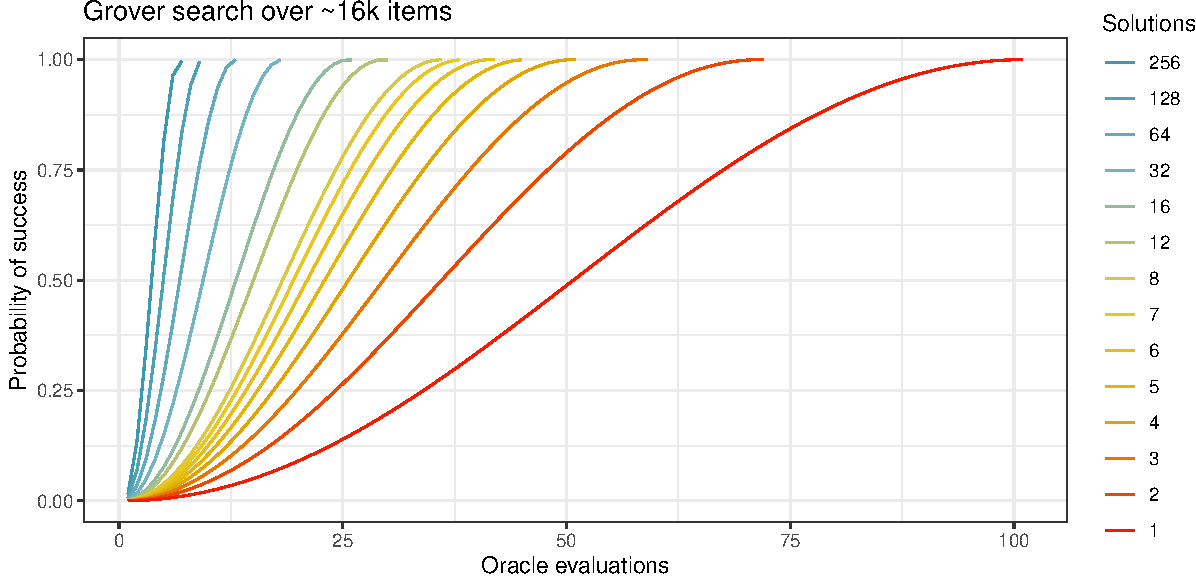
\includegraphics[width=0.9\linewidth]{groverCurves.pdf}
	\caption{Curves depict the probability that Grover's quantum search algorithm returns a solution as a function of the number of oracle evaluations. For the ranges depicted, the number of iterations required and the number of solutions inversely relate, but increasing the number of iterations past \emph{R} (Equation \ref{eq:R}) can backfire and lead to extremely small probabilities of success.  }\label{fig:grov}
\end{figure}

Given a set of $N$ items and a function $f:\{0,1,\dots,N-1\}\rightarrow \{0,1\}$ that evaluates to $1$ for a single element, \citet{grover1996fast} develops an algorithm that uses quantum parallelism to score quadratic speedups over its classical counterparts. After only $\mathcal{O}(\sqrt{N})$ evaluations of $f(\cdot)$, Grover's algorithm returns the $x\in \{0,1,\dots,N-1\}$ satisfying $f(x) =1$ with high probability.  Compare this to $\order{N}$ requirement for the randomized classical algorithm that must evaluate $f(\cdot)$ over at least $N/2$ items to obtain the same probability of detecting $x$.  The algorithm takes the state $\ket{0}^{\otimes N}\ket{1}$ as input and applies Hadamard gates to each of the individual $N+1$ input qubits.  The resulting state is 
\begin{align*}
\ket{h}\ket{-}= \left(\frac{1}{\sqrt{N}} \sum_{x=0}^{N-1} \ket{x} \right)  \frac{1}{\sqrt{2}}\left(\ket{0} -\ket{1}\right) =  \frac{1}{\sqrt{N}} \sum_{x=0}^{N-1} \ket{x} \ket{-} \, .
\end{align*}
Next, we apply the oracle gate $\U_f: \ket{x}\ket{y} \rightarrow \ket{x}\ket{y\oplus f(x)}$ and note that 
\begin{align*}
\U_f \ket{x} \ket{-} &= \U_f \ket{x} \frac{1}{\sqrt{2}}\left(\ket{0} -\ket{1}\right) 
= \frac{1}{\sqrt{2}} \big(\ket{x} \ket{0\oplus f(x)} - \ket{x}\ket{1\oplus f(x)} \big) \\
&= -1^{f(x)} \ket{x}\ket{-}  \, .
\end{align*}
Thus, $\U_f$ flips the sign for the state $\ket{x_0}$ for which $f(x_0)=1$ but leaves the other states unchanged.  If we suppress the ancillary qubit $\ket{-}$, then $\U_f$ is equivalent to the gate $\U_{x_0}$ defined as $\U_{x_0} \ket{x} = -1^{\delta_{x_0}}\ket{x}$. We may succinctly write this gate as the Householder matrix that reflects vectors about the unique hyperplane through the origin that has $\ket{x_0}$ for a normal vector:
\begin{align*}
\U_{x_0}= \I - 2 \ket{x_0}\bra{x_0} \, .
\end{align*}
The action of this gate on the state $\ket{h}$ takes the form
\begin{align*}
\frac{1}{\sqrt{N}} \sum_{x=0}^{N-1} \ket{x} \longrightarrow \frac{1}{\sqrt{N}} \sum_{x=0}^{N-1} -1^{\delta_{x_0}(x)} \ket{x} \, .
\end{align*}
Next, the algorithm reflects the current state about the hyperplane that has $\ket{h}$ as a normal vector and negates the resulting state:
\begin{align*}
\Big(2\ket{h}\bra{h}-\I \Big) \left( \frac{1}{\sqrt{N}} \sum_{x=0}^{N-1} -1^{\delta_{x_0}(x)} \ket{x}  \right)
&= \frac{1}{\sqrt{N}}\sum_{x} \left( (-1)^{1-\delta_{x_0}(x)} + 2 \frac{(N-2)}{N} \right)\ket{x}\\ &= \frac{(3N-4)}{N^{3/2}} \ket{x_0} + \sum_{x\neq x_0} \frac{(N-4)}{N^{3/2}}  \ket{x} \, .
\end{align*}
The scientist who measures the state at this moment would obtain the desired state $\ket{x_0}$ with a slightly higher probability of $(3N-4)^2/N^3$  than the individual probabilities of $(N-4)^2/N^3$ for the other states. Each additional application of the \emph{Grover iteration}
\begin{align*}
\G := - \U_h \U_{x_0} := \Big(2\ket{h}\bra{h}-\I \Big) \Big( \I - 2 \ket{x_0}\bra{x_0} \Big)
\end{align*}
increases the probability of obtaining $\ket{x_0}$ at the time of measurement in the computational basis and $R=\ceil{\pi\sqrt{N}/4}$ iterations guarantees a probability of success that is greater than $1-1/N$.

  \begin{algorithm}[th!]
	\caption{Quantum exponential searching algorithm \citep{boyer1998tight}}\label{alg:expoSearch}
	\KwData{An oracle gate $\U_f$ taking $\ket{x}\ket{y}$ to $\ket{x}\ket{y\oplus f(x)}$ for a function $f(x):\{0,\dots,N-1\}\rightarrow \{0,1\}$ with unknown number of solutions; $n=\log_2(N)$.}
	\KwResult{If a solution exists, an $n$-bit binary string $x_0$ satisfying $f(x_0)=1$; if no solution exists, the algorithm runs forever.}
	$m \gets 1$\;
	$\gamma \gets 6/5$\;
	success $\gets$ \textcolor{blue}{FALSE}\;
	\While{\emph{success}$\neq$\emph{\textcolor{blue}{TRUE}}}{
		$j \gets Uniform \{0,\cdots,m-1\}$\;
		$\ket{0}^{\otimes n}\ket{1} \longrightarrow \H^{\otimes n+1}\ket{0}^{\otimes n}\ket{1}= \ket{h}\ket{-}$\; 
		$\ket{h}\ket{-} \longrightarrow \G^j \ket{h}\ket{-} = \ket{x}\ket{-}$;\hspace{1em}  \Comment{$j$ Grover iterations from Alg \ref{alg:grover}.}  
		$\ket{x} \longrightarrow x$; \hspace{16em} \Comment{Measure and check.}  
		\uIf{$f(x)=1$}{$x_0 \gets x$\;
			success $\gets$  \textcolor{blue}{TRUE}\;}
		\Else{$m \gets \min\left( \gamma m, \sqrt{N}\right)$;\hspace{4em}  \Comment{Increase $m$ in case of failure.}
	}}
	\Return{$x_0$}\ .
	
	\vspace{0.5em}
\end{algorithm}

In general, we may use Grover's search algorithm to find a solution when the number of solutions $M$ is greater than 1. While the algorithmic details change little, the number of required Grover iterations
\begin{align}\label{eq:R}
R = \ceil[\Bigg]{\frac{\pi}{4} \sqrt{\frac{N}{M}}}
\end{align}
 and the probability of success after those $R$ iterations \emph{do} change \citep{boyer1998tight}.  When $M$ is much smaller than $N$, the success rate is greater than $1-M/N$, and even for large $M$ the success rate is more than $1/2$. Lower-bounds are useful for establishing mathematical guarantees, but it is also helpful to understand the quality of algorithmic performance as a function of $M$ and $R$. Figure \ref{fig:grov} shows success curves as a function of the number of Grover iterations (or oracle calls) applied.  The search field contains $2^{14} \approx 16$k elements, and the number of solutions $M$ varies. Each curve represents an individual search task.  The algorithm requires more iterations for smaller numbers and fewer iterations for larger numbers of solutions.  The upper bound on error $M/N$ is only an upper bound: the final probability of success for, e.g., $M=256$ is 0.997 compared to the bound of 0.984.
 

 
 While Grover's algorithm delivers impressive speedups over classical search algorithms, it has a major weakness.
 Figure \ref{fig:grov} hides the fact that the probability of success for Grover's algorithm is \emph{not} monatonic in the number of iterations.  Running the algorithm for more than $R$ iterations can backfire.  For example, running the algorithm for $\sqrt{2N}$ iterations when $M=1$ results in a probability of success less than $0.095$ \citep{boyer1998tight}.  The non-monotinicity of Grover's algorithm becomes particularly problematic when we do not know the number of solutions $M$. Taking for example $N=2^{20}$, \citet{boyer1998tight} point out that 804 iterations provide an extremely high probability of success when $M=1$ but a one-in-a-million chance of success when $M=4$.  To solve this problem and develop an effective search algorithm when $M$ is unknown, those authors adopt the strategy of focusing on the expected number of iterations before success. In particular, they propose the quantum exponential search algorithm (Algorithm \ref{alg:expoSearch}).  When a solution exists, the algorithm returns a solution with expected total number of Grover iterations bounded above by $\frac{9}{2}\sqrt{N/M}$.  Still better, this upper bound reduces to $\frac{9}{4}\sqrt{N/M}$ for the special case $M\ll N$, and simulations presented in Figure \ref{fig:expo} show that even this bound is large.  Such results come in handy when deciding whether to halt the algorithm's progress if one believes it possible that no solutions exist.  Indeed, this turns out to be useful in the context of quantum minimization.
 

 
 \begin{figure}[!t]
 	\centering
 	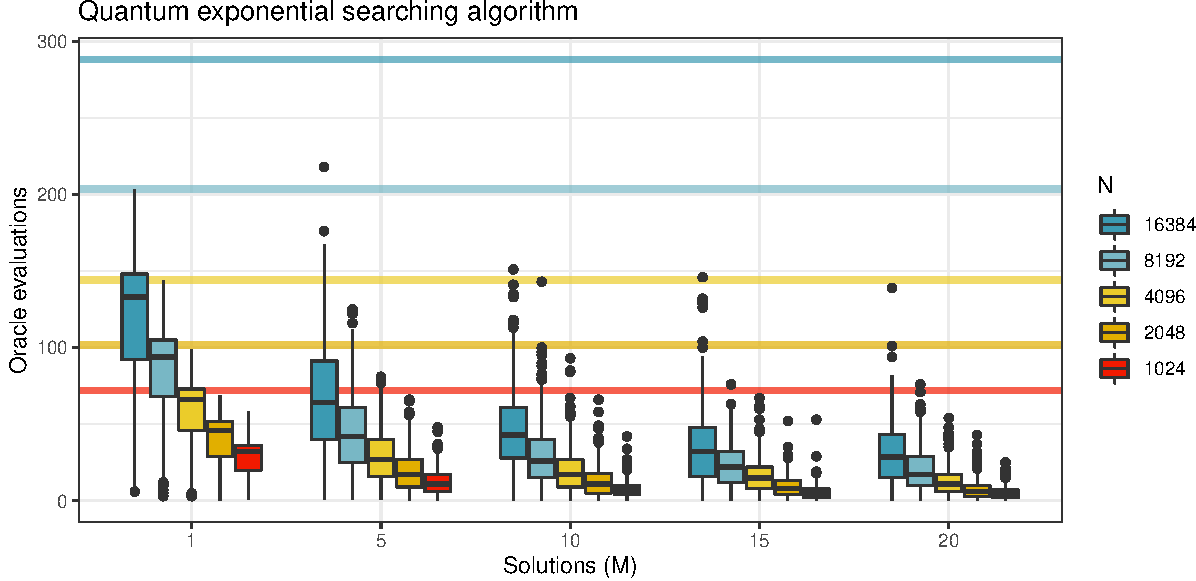
\includegraphics[width=0.9\linewidth]{expoSearch.pdf}
 	\caption{Total number of oracle evaluations required by quantum exponential searching algorithm \citep{boyer1998tight} for different numbers of solutions $M$ and search set sizes $N$ from 500 independent simulations each.  Horizontal lines at $\frac{9}{4}\sqrt{N}$ represent upper bounds on expected total number of evaluations to obtain a solution for the $M=1$ problem.}\label{fig:expo}
 \end{figure}
 

 
 \subsection{Quantum minimization}

 \begin{figure}[!t]
	\centering
	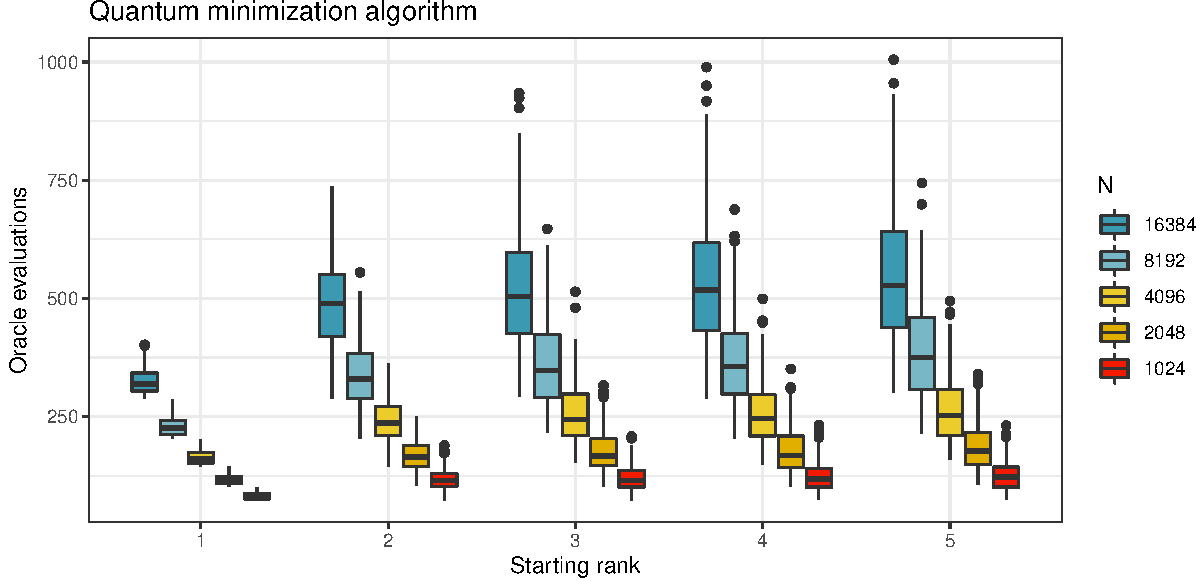
\includegraphics[width=0.9\linewidth]{qMinAlg.pdf}
	\caption{Total number of oracle evaluations required by quantum minimization algorithm \citep{durr1996quantum} for different starting ranks and search set sizes $N$ from 500 independent simulations each.  Less than 1\% of the 12,500 instances failed to recover the true minimum.}\label{fig:qMinAlg}
\end{figure}

 \begin{algorithm}[t!]
	\caption{Quantum minimum searching algorithm \citep{durr1996quantum}}\label{alg:min}
	\KwData{An unordered database $T[0,\dots,N-1]$ with unique integer elements; a maximum error tolerance $err\in(0,1)$; expected time to success $m_0=\frac{45}{4}\sqrt{N}+\frac{7}{10}\log_2(N)$.}
	\KwResult{An $n$-bit binary string $x_0$ satisfying $T[x_0] = \min T$ with probability greater than $1-\epsilon$.}
	$s \gets 0$\;
	$x_0 \gets Uniform\{0,\dots,N-1\}$\;
	\While{$s< m_0/\epsilon$}{
		Prepare initial state $\frac{1}{\sqrt{N}}\sum_x\ket{x}\ket{x_0}$\;
		Mark all items $x$ satisfying $T[x]<T[x_0]$\;
		$s\gets s+ \log_2(N)$\;
		Apply quantum exponential searching algorithm (Alg \ref{alg:expoSearch}); \Comment{$I$ timesteps}
		$s\gets s+ I$\;
		Obtain $x'$ by measuring first register\;
		\If{$T[x']<T[x_0]$}{$x_0 \gets x'$}
	}
	\Return{$x_0$} \ .
		\vspace{0.5em}
		
\end{algorithm}

Given a function $f(\cdot)$ that maps the discrete set $\{0,\dots,N-1\}$ to the integers, we wish to find the minimizer
\begin{align*}
x_0 = \argmin_{x\in\{0,\dots,N-1\}} f(x) \, .
\end{align*}
 \citet{durr1996quantum} propose a quantum algorithm for finding $x_0$ that iterates between updating a running minimum $F\in f(\{0,\dots,N-1\})$ and applying the quantum exponential search algorithm (Algorithm \ref{alg:expoSearch}) to find an element $x$ such that $f(x)<F$.  Having run these iterations a set number of times, the algorithm returns the minimizer $x_0$ with high probability. 
 To this end, \citet{durr1996quantum} show that their algorithm takes an expected total time of $m_0=\frac{45}{4}\sqrt{N}+\frac{7}{10}\log_2(N)$ to find the minimizer, where marking items with values less than the threshold value (Algorithm \ref{alg:min}) requires $\log_2(N)$ time steps and each Grover iteration within the quantum exponential search algorithm requires one time step. From there, Markov's inequality says
 \begin{align*}
 \mbox{Pr}\left( \mbox{total time to success} \geq \frac{m_0}{\epsilon}\right) \leq \frac{\mbox{E}\left(\mbox{total time to success}\right)}{m_0/\epsilon}=\epsilon \, ,
 \end{align*}
 or that we must scale the minimization procedure's time steps by a factor of $1/\epsilon$ to reach a failure rate less than $\epsilon$.

\begin{lemma}[Warm-starting]\label{lem:warm}
	Suppose that the quantum minimization algorithm begins with a threshold $F_0$ such that $f(x)<F_0$ for only $K-1$ items. Then the expected total number of time steps to find the minimizer is bounded above by
	\begin{align*}
	m_0^K = \left(\frac{5}{4} - \frac{1}{\sqrt{K-1}} \right) 9\sqrt{N} + \frac{7}{10} \log_2(K) \log_2(N) \, ,
	\end{align*}
	and so the following rule relates the warm-started upper bound to the generic upper bound:
	\begin{align*}
	m_0^K = m_0 - 9\sqrt{\frac{N}{K-1}} + \frac{7}{10} \log_2 \left(\frac{K}{N} \right) \log_2(N)\, .
	\end{align*} 
\end{lemma}
\begin{proof}
	The proof follows the exact same form as Lemma 2 of \citet{durr1996quantum}. It relies on a theoretical algorithm called the \emph{infinite algorithm} that runs until the minimum is found.  In this case, Lemma 1 of that paper says that the probability that the $r$th lowest value is ever selected when searching among $K$ items is $p(K,r)=1/r$ for $r\leq K$ and 0 otherwise.  For a warm-start at element $K$, the expected total time spent in the exponential search algorithm is
	\begin{align*}
	\sum_{r=2}^N p(K,r) \frac{9}{2} \sqrt{\frac{N}{r-1}} &= \sum_{r=2}^K p(K,r) \frac{9}{2} \sqrt{\frac{N}{r-1}} 
	=  \frac{9}{2}\sqrt{N}\sum_{r=1}^{K-1} \frac{1}{r+1} \frac{1}{\sqrt{r}} \\
	&\leq \frac{9}{2}\sqrt{N}\left( \frac{1}{2}+\sum_{r=2}^{K-1} r^{-3/2} \right) \leq \frac{9}{2}\sqrt{N}\left( \frac{1}{2}+\int_{r=1}^{K-1} r^{-3/2} \dd r \right) \\
	&= \left(\frac{5}{4} - \frac{1}{\sqrt{K-1}} \right) 9\sqrt{N} \, .
	\end{align*}
	An upper bound for the expected total number of time steps preparing the initial state and marking items $T[x]<T[x_0]$ follows in a similar manner.
\end{proof}

Lemma \ref{lem:warm} shows that, e.g., if Algorithm \ref{alg:min} begins at the item with second lowest value, then the expected total time to success is bounded above by $m_0^2=\frac{9}{4}\sqrt{N}+\frac{7}{10}\log_2(N)$, reducing the generic upper bound by $9\sqrt{N}-\frac{7}{10}\log_2\left( \frac{2}{N}\right)\log_2(N)$ time steps.  When $N$ equals 1000, say, the expected total time steps is $m_0^2< 78.2$.  Keeping $N=1000$ but letting the algorithm begin at the third lowest value ($K=3$), the expected total time steps before success is $m_0^3<165.6$. Raising $N$ to 10,000, the two numbers increase to $m_0^2< 234.4$ and $m_0^3<503.4$. These warm-starting upper bounds on the expected total time needed to obtain the minimum are especially useful in the context of parallel MCMC, when the current state $\ttheta^{(s)}$ inhabits the high-density region of the target distribution but the \emph{vast} majority of proposals do not.  

%Indeed, the empirically optimal rejection rate for, e.g., the simplicial sampler of \citet{holbrook2021generating} reaches a \emph{minimum} of approximately 0.35 in high-dimensions: for roughly a third of the MCMC iterations, the current state 

\section{Quantum parallel MCMC}

With the rudiments of quantum minimization in hand, we present our quantum parallel parallel MCMC (qp$^2$MCMC). The general structure of the algorithm is the same as that of other parallel MCMC algorithms: the algorithm generates a Markov chain by iterating between proposing and selecting new Markov chain states.  Unlike classical single-proposal MCMC, parallel MCMC proposes many states and chooses one according to the generalized acceptance probabilities of Equation \eqref{eq:probs}:
\begin{align*}
\pi_j = \frac{\pi(\ttheta_j) \prod_{k \neq j} q(\ttheta_j,\ttheta_k)}{\sum_{i=0}^K \pi(\ttheta_i) \prod_{k \neq i} q(\ttheta_i,\ttheta_k)} \, , \quad j=0,\dots,K \, .
\end{align*}
 In general MCMC, evaluation of the target density function $\pi(\cdot)$ is the rate-limiting computational step, becoming particularly onerous in big data scenarios.  While parallel MCMC benefits from improved mixing as a function of MCMC iterations, the increased computational burden of $P$ target evaluations at each step can lead to less favorable comparisons when accounting for elapsed wall-clock time.
 
 \emph{Having successfully generated proposals $\ttheta_j,$ $j=1,\dots,P$ and evaluated the corresponding densities $q(\cdot,\cdot)$, we would like to use quantum parallelism and an oracle gate (say, $\U_\pi$) to efficiently compute the $\pi(\ttheta_j)$s but immediately encounter a Catch-22 when we seek to draw a sample $\ttheta^{(s+1)} \sim$ \emph{Discrete}$(\pi_0,\pi_1,\dots,\pi_P)$.  We can use neither a quantum nor a classical circuit to draw the sample! On the one hand, drawing the sample within a quantum circuit would somehow require that all superposed states have access to all the $\pi(\ttheta_j)$s at once to perform the required normalization.  On the other hand, drawing the sample within the classical circuit would require access to all the $\pi(\ttheta_j)$s, but measurement in the computational basis can only return one.}  
 
 In light of this dilemma, we propose to use the Gumbel-max trick to transform the generalized accept-reject step into a discrete optimization procedure.  From there, we use quantum minimization to efficiently sample from $\ppi$. Crucially, we get away with quantum parallel evaluation of the target $\pi(\cdot)$ over all superposed states because the Gumbel-max trick does not rely on a normalization step: each superposed state requires no knowledge of any target evaluation other than its own.  
 
 
%qp$^2$MCMC uses quantum minimization to limit the number of target evaluations within the generalized acceptance step with the help of the Gumbel-max trick, which transforms the discrete sampling task $\ttheta^{(s+1)} \sim$ Discrete$(\pi_0,\pi_1,\dots,\pi_P)$ into a search problem over a discrete set of real numbers. 

\subsection{Gumbel-max}\label{sec:gm}
\newcommand{\p}{\mbox{p}}

We wish to randomly select a single element from the set $\{0,1,\dots,P\}$ with probability proportional to the unnormalized probabilities $\ppi^*=(\pi_0^*,\pi_1^*,\dots,\pi_P^*)$.  That is, there exists a $c>0$ such that $\ppi^* = c \ppi$, for $\ppi$ a valid probability vector, but we only have access to $\ppi^*$.  Define $\llambda:= \log \ppi$ and $\llambda^*:= \log \ppi^*=\log\ppi + \log c$,  and assume that $z_0,\dots,z_P\stackrel{iid}{\sim}Gumbel(0,1)$. Then, the probability density function $g(\cdot)$ and cumulative distribution function $G(\cdot)$ for each individual $z_p$ are
\begin{align}
g(z_p) = \exp\big(-z_p- \exp(-z_p)\big) \, , \quad \mbox{and} \quad G(z_p) = \exp \big( -\exp(-z_p) \big)\, .
\end{align}
Now, defining the random variables $\alpha^*_p:=\lambda^*_p+z_p$, $\alpha_p:=\lambda_p+z_p$ and  
\begin{align}
\hat{p} = \argmax_{p=0,\dots,P}\: \alpha^*_p \, ,
\end{align}
we have the result
\begin{align}
\mbox{Pr} (\hat{p} = p) = \pi_p \, .
\end{align}
In words, the procedure of adding Gumbel noise to unnormalized log-probabilities and taking the index of the maximum produces a random variable that follows the discrete distribution over $\ppi$.  Moving from left to right:
\begin{align*}
\mbox{Pr} (\hat{p} = p) &= \mbox{Pr} (\alpha^*_p > \alpha^*_{p'}, \, \forall p' \neq p ) \\
&= \mbox{Pr} (\alpha_p +\log c > \alpha_{p'} + \log c, \, \forall p' \neq p ) 
= \mbox{Pr} (\alpha_p  > \alpha_{p'} , \, \forall p' \neq p ) \\
&= \int_{-\infty}^\infty \prod_{p'\neq p} \mbox{Pr} (\alpha_p > \alpha_{p'}| \alpha_p) g(\alpha_p-\lambda_p) \, \dd \alpha_p 
= \int_{-\infty}^\infty \prod_{p'\neq p} G(\alpha_p-\lambda_{p'}) g(\alpha_p-\lambda_p) \, \dd \alpha_p \\
&=  \int_{-\infty}^\infty  \prod_{p'\neq p} \exp\big( -\exp(\lambda_{p'}-\alpha_p)\big) \exp\big(-\alpha_p+\lambda_p - \exp(-\alpha_p+\lambda_p) \big) \, \dd \alpha_p \, .
\end{align*}
Recalling that $\lambda_{p'}=\log \pi_{p'}$, we exponentiate the logarithms, and the integral becomes
\begin{align*}
& \pi_p \int_{-\infty}^\infty  \prod_{p'\neq p} \exp\big( -\pi_{p'}\exp(-\alpha_p)\big) \exp  \big(-\alpha_p - \pi_p\exp(-\alpha_p) \big) \, \dd \alpha_p \\
&= \pi_p \int_{-\infty}^\infty \exp  (-\alpha_p ) \exp\big( -\sum_{p'=0}^P\pi_{p'}\exp(-\alpha_p)\big)  \, \dd \alpha_p  \\
&= \pi_p \int_{-\infty}^\infty \exp  (-\alpha_p ) \exp\big( -\exp(-\alpha_p)\big)  \, \dd \alpha_p  = \pi_p \, ,
\end{align*}
where the final equality follows easily from the change of variables $u=\exp(-\alpha_p)$.  


\begin{algorithm}
	\caption{The Gumbel-max trick}\label{alg:gm}
	\KwData{A vector of unnormalized log-probabilities $\llambda^*=\log \ppi +\log c$, for $\ppi$ a discrete probability vector with $P+1$ elements.}
	\KwResult{A single sample $p \sim$ \emph{Discrete}$(\ppi)$ satisfying $p\in\{0,1,\dots,P\}$.}
	\For{$p' \in\{0,1,\dots,P\}$}{
		$z_{p'} \gets Gumbel(0,1)$\;
		$\alpha^*_{p'} \gets \lambda_{p'}^* + z_{p'}$\;
	}
	$p \gets \argmax_{p'=0,\dots,P}\alpha^*_{p'}$\;
	\Return{p}\ .
	
	\vspace{0.5em}
\end{algorithm}


\subsection{QPMCMC}

 \begin{figure}[!t]
	\centering
	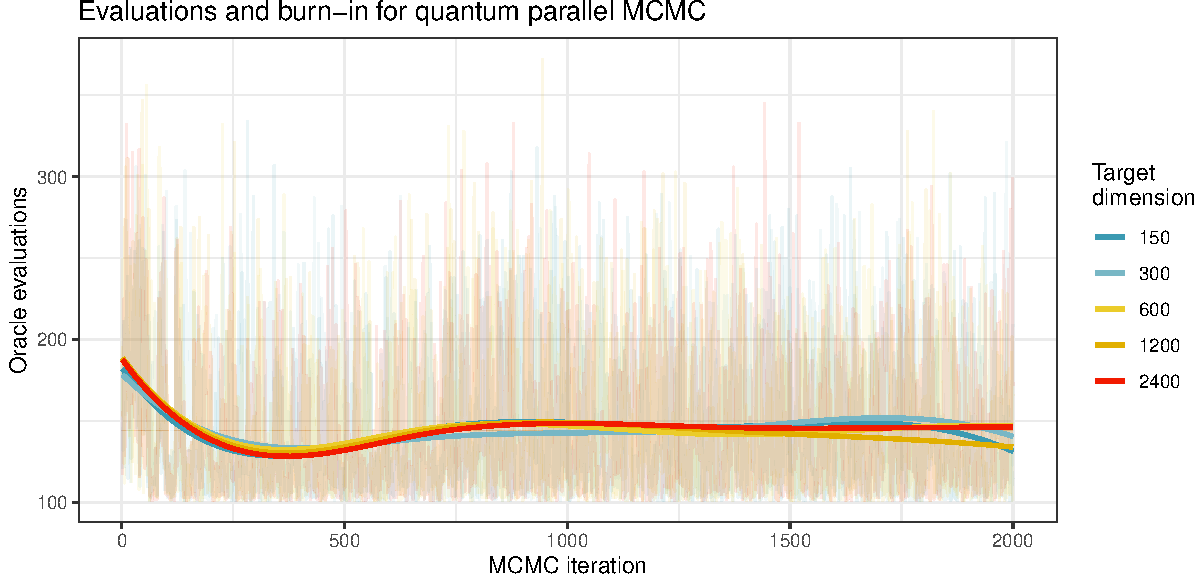
\includegraphics[width=0.9\linewidth]{mcmcIterations.pdf}
	\caption{Total number of oracle evaluations required for each of 2,000 parallel MCMC iterations. In total, the combined MCMC runs required roughly $7$\% of the usual 20 million target evaluations. Over  99.4\% of the 10,000 MCMC iterations successfully sampled from the discrete distribution with probabilities of Equation \eqref{eq:probs}.}\label{fig:mcmcIterations}
\end{figure}

\begin{algorithm}[t!]
	\caption{Quantum parallel parallel MCMC}\label{alg:qpMCMC}
	\KwData{Initial Markov chain state $\ttheta^{(0)}$; total length of Markov chain $S$; total number of proposals per iteration $P$; routine for evaluating target density $\pi(\cdot)$; routines for drawing random samples from the proposal distribution $Q(\ttheta^{(s)},\cdot)$ and the standard Gumbel distribution $Gumbel(0,1)$.}
	\KwResult{A Markov chain $\ttheta^{(1)}, \dots, \ttheta^{(S)}$.}
	\For{$s \in\{1,\dots,S\}$}{
		%$\sigma_\pi \gets 0$\;
		$\ttheta_0 \gets \ttheta^{(s-1)}$\;
		\For{$p' \in \{1,\dots,P\}$}{
			$\ttheta_{p'} \gets Q(\ttheta^{(s-1)},\cdot)$\;
		}
		\For{$p' \in \{0,\dots,P\}$}{
			$q_{p'} \gets  \prod_{p''\neq p'}q(\ttheta_{p'},\ttheta_{p''})$\; 
			$z_{p'} \gets Gumbel(0,1)$\;
		}
		$p \gets \argmin_{p'=0,\dots,P}f(p')= -\left(\log \big(\pi(\ttheta_{p'}) q_{p'}\big) + z_{p'}\right)$; \hspace{2em} \Comment{$\order{\sqrt{P}}$ Alg \ref{alg:min}}
		$\ttheta^{(s)} \gets \ttheta_p$\;
	}
	\Return{$\ttheta^{(1)}, \dots, \ttheta^{(S)}$}\ .
	
		\vspace{0.5em}
\end{algorithm}


 \begin{figure}[!h]
	\centering
	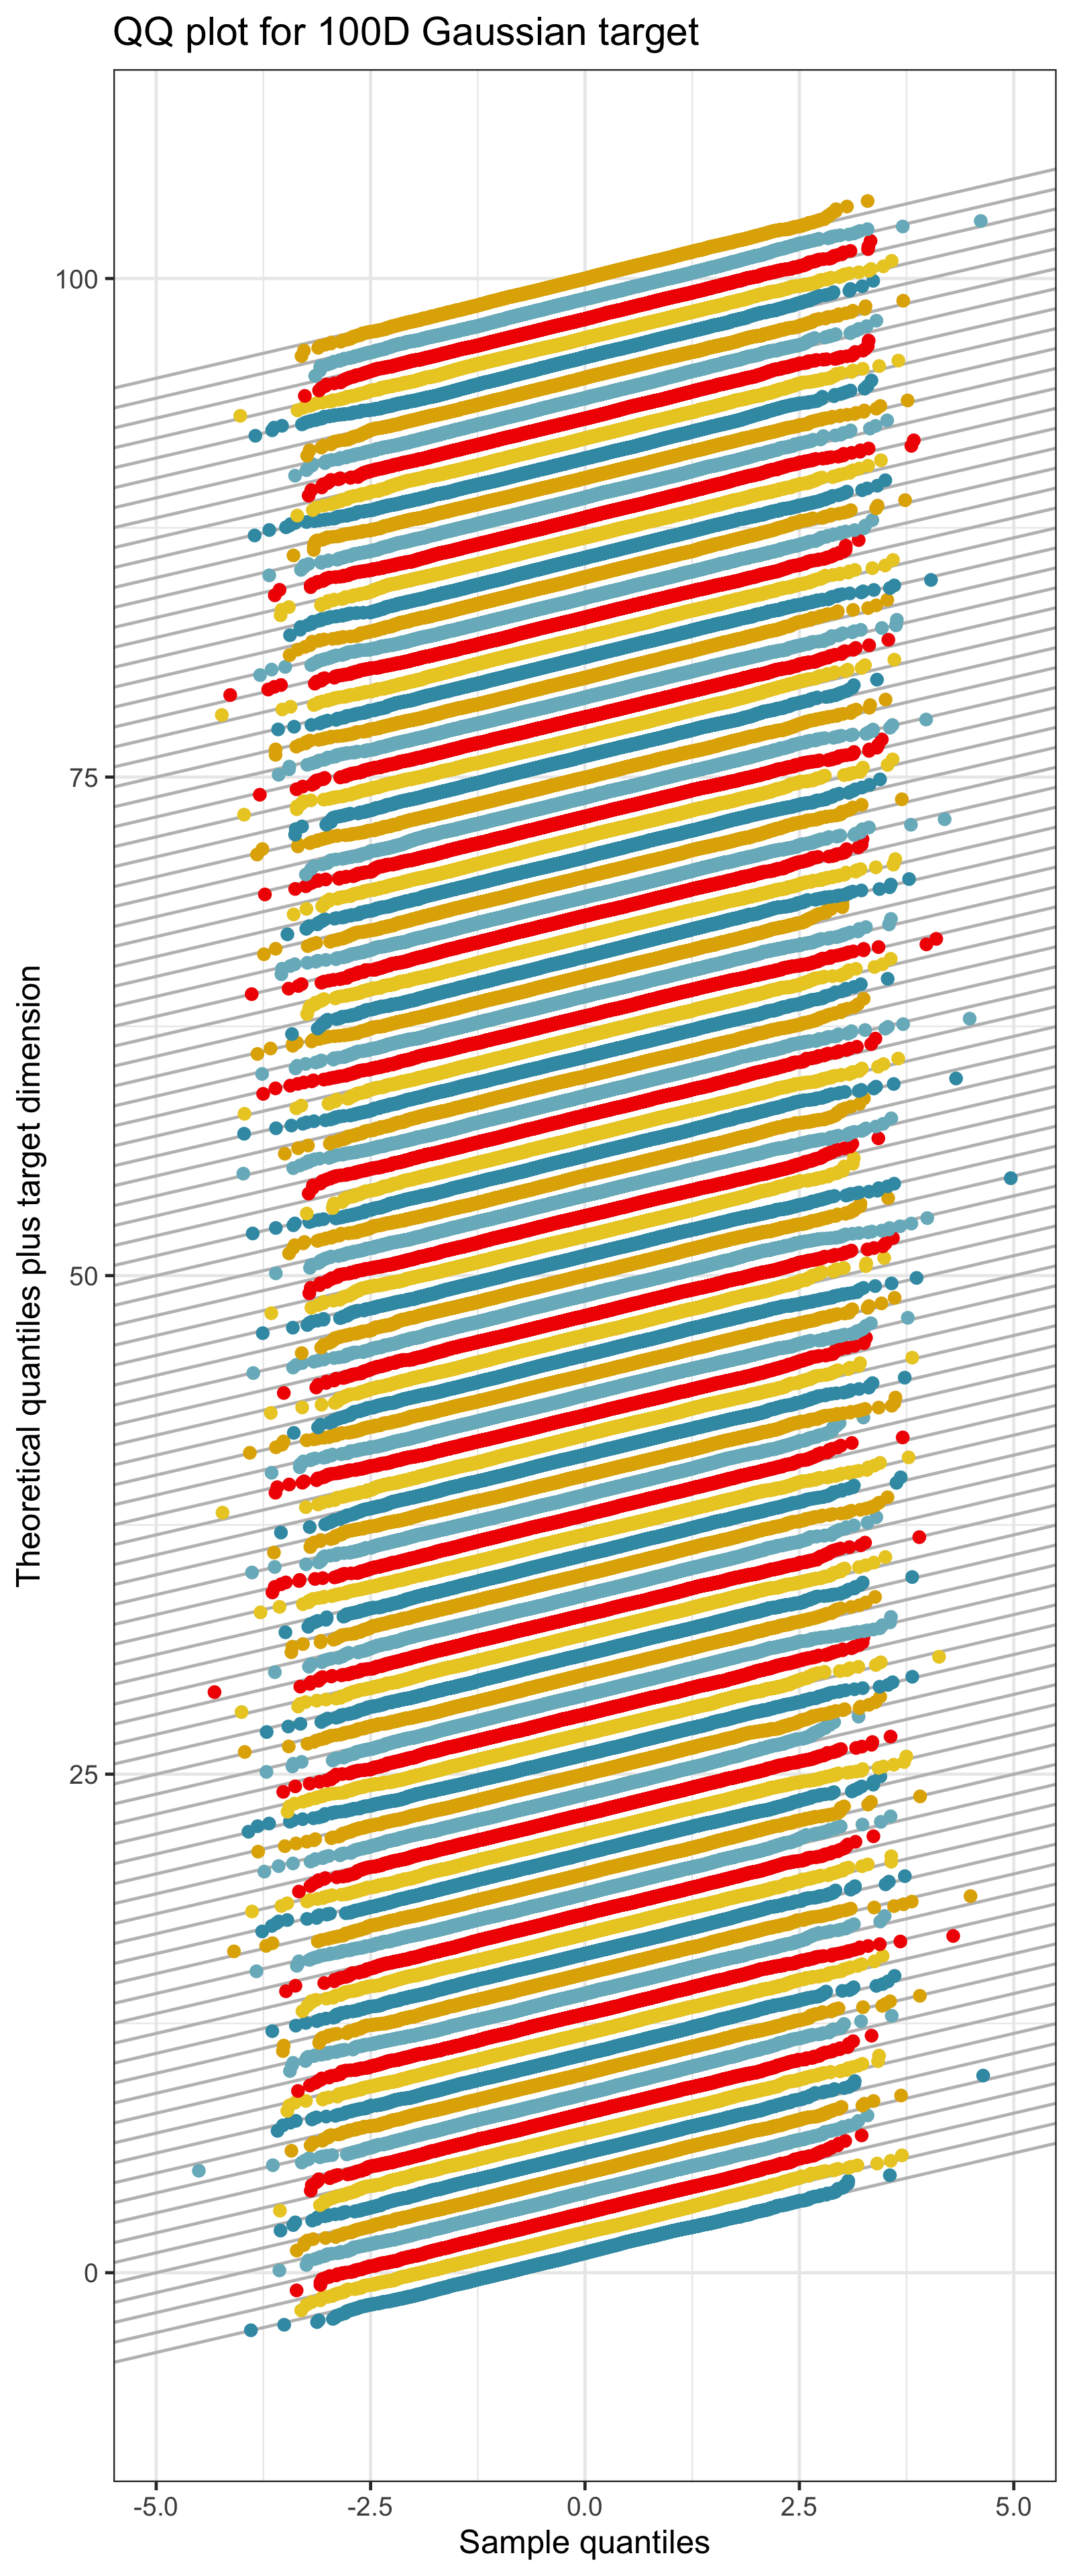
\includegraphics[width=0.5\linewidth]{qqPlot.png}
	\caption{Empirical accuracy of quantum parallel MCMC (QPMCMC) for a 100 dimensional spherical Gaussian target.  We generate 100,000 samples using 2,000 proposals each iteration and remove the first 2,000 samples as burn-in.  The QQ (quantile-quantile) plot shows sample quantiles adhering closely to the theoretical quantiles.  Similar to the independent simulation shown in Figure \ref{fig:mcmcIterations}, here QPMCMC requires less than $7.2$\% of the usual number of target evaluations.}\label{fig:qq}
\end{figure}

\section{Reading the fine print}

\bibliographystyle{sysbio}
\bibliography{refs}

\appendix




%%%%%%%%%%%%%%%%%%%%%%%%%%%%%%%%%%%%%%%%%%%%%%%%%%%%%%%%%%%%

\end{document}
